%!TEX root = ../effc_top.tex

\begin{frame}[fragile]{Proof}
	\colorit{Basic case:} $\cM(s,0) \cong \Z\{
	\raisebox{-3pt}{
		\begin{tikzpicture}[scale=.3]
			\draw (0,.5)--(0,-.75);
			\node[scale=.4] at (0,.75){1};
			\fill (0,-.65) circle (3pt);

			\node[scale=.4] at (.55,0){$\dots$};

			\draw (1,.5)--(1,-.75);
			\node[scale=.5] at (1,.75){$s$};
			\fill (1,-.65) circle (3pt);
		\end{tikzpicture}
	}\}$

	\medskip\pause

	\colorit{Contraction:} $\bd \circ \, h = \id - p \circ i + h \circ \bd$
	\vskip -5pt
	\[
	\begin{tikzcd}
		\cM(s,r-1) \arrow[r, "i", shift left=3pt]
		& \cM(s,r) \arrow[l, "p", shift left=3pt] \arrow[loop right, "h", distance=2em]
	\end{tikzcd}
	\]
	\pause\vskip -20pt
	\[
	\begin{tikzpicture}[scale=.3]
		\draw (0,1) -- (0,-1);
		\draw (1,1) -- (1,-1);
		\draw (0,.5) -- (1,.5);
		\draw (0,-.5) -- (1,-.5);
		\node[scale=.4] at (0,1.25){$1$};
		\node[scale=.4] at (0,-1.25){$1$};
		\node[scale=.4] at (1,1.25){$s$};
		\node[scale=.4] at (1,-1.25){$r-1$};
		\draw (1.5,0) edge[|->] (5.5,0);
	\end{tikzpicture}
	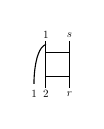
\begin{tikzpicture}[scale=.3]
		\draw (0,1) -- (0,-1);
		\draw (1,1) -- (1,-1);
		\draw (0,.5) -- (1,.5);
		\draw (0,-.5) -- (1,-.5);
		\node[scale=.4] at (0,1.25){$1$};
		\node[scale=.4] at (0,-1.25){$2$};
		\node[scale=.4] at (1,1.25){$s$};
		\node[scale=.4] at (1,-1.25){$r$};
		\draw (0,.85) edge[out=200,in=-90] (-.5,-.7);
		\node[scale=.4] at (-.5,-1.25){$1$};
	\end{tikzpicture}
	\]
	\vskip -10pt
	\[
	\begin{tikzpicture}[scale=.3]
		\node at (-7.5,0){};
		\draw (-5,1) -- (-5,-1);
		\draw (-6,1) -- (-6,-1);
		\draw (-6,.5) -- (-5,.5);
		\draw (-6,-.5) -- (-5,-.5);
		\node[scale=.4] at (-6,1.25){$1$};
		\fill (-6,-.95) circle (3pt);
		\node[scale=.4] at (-5,1.25){$s$};
		\node[scale=.4] at (-5,-1.25){$r-1$};
		\draw (-4.5,0) edge[<-|] (-.5,0);
		%%%%%%%%%%%%%%%%%%%%%%%%%%%%%%%%%
		\draw (0,1) -- (0,-1);
		\draw (1,1) -- (1,-1);
		\draw (0,.5) -- (1,.5);
		\draw (0,-.5) -- (1,-.5);
		\node[scale=.4] at (0,1.25){$1$};
		\node[scale=.4] at (0,-1.25){$1$};
		\node[scale=.4] at (1,1.25){$s$};
		\node[scale=.4] at (1,-1.25){$r$};
		\draw (1.5,0) edge[out=0,in=0,|->] (1.5,-4);
		%%%%%%%%%%%%%%%%%%%%%%%%%%%%%%%%%
		\draw (0,-3) -- (0,-5);
		\draw (1,-3) -- (1,-5);
		\draw (0,-3.5) -- (1,-3.5);
		\draw (0,-4.5) -- (1,-4.5);
		\node[scale=.4] at (0,-2.75){$1$};
		\node[scale=.4] at (0,-5.25){$1$};
		\node[scale=.4] at (1,-2.75){$s$};
		\node[scale=.4] at (1,-5.25){$r$};
		\draw (0,-3.15) edge[out=200,in=160] (0,-4.85);
	\end{tikzpicture}
	\]
	\pause\vskip -25pt\colorit{Then}
	\[
	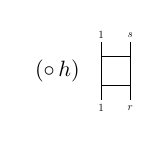
\begin{tikzpicture}[scale=.37]
		\node[scale=.8] at (-1.5,0){$(\bd \circ \, h)$};
		\draw (0,1) -- (0,-1);
		\draw (1,1) -- (1,-1);
		\draw (0,.5) -- (1,.5);
		\draw (0,-.5) -- (1,-.5);
		\node[scale=.4] at (0,1.25){$1$};
		\node[scale=.4] at (0,-1.25){$1$};
		\node[scale=.4] at (1,1.25){$s$};
		\node[scale=.4] at (1,-1.25){$r$};
	\end{tikzpicture}
	\pause
	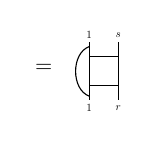
\begin{tikzpicture}[scale=.37]
		\node[scale=.8] at (-1.5,.1){$= \, \bd $};
		\draw (0,1) -- (0,-1);
		\draw (1,1) -- (1,-1);
		\draw (0,.5) -- (1,.5);
		\draw (0,-.5) -- (1,-.5);
		\node[scale=.4] at (0,1.25){$1$};
		\node[scale=.4] at (0,-1.25){$1$};
		\node[scale=.4] at (1,1.25){$s$};
		\node[scale=.4] at (1,-1.25){$r$};
		\draw (0,.85) edge[out=200,in=160] (0,-.85);
	\end{tikzpicture}
	\pause
	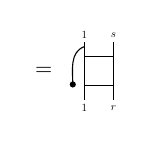
\begin{tikzpicture}[scale=.37]
		\node[scale=.8] at (-1.4,0){$=$};
		\draw (0,1) -- (0,-1);
		\draw (1,1) -- (1,-1);
		\draw (0,.5) -- (1,.5);
		\draw (0,-.5) -- (1,-.5);
		\node[scale=.4] at (0,1.25){$1$};
		\node[scale=.4] at (0,-1.25){$1$};
		\node[scale=.4] at (1,1.25){$s$};
		\node[scale=.4] at (1,-1.25){$r$};
		\draw (0,.85) edge[out=200,in=90] (-.4,-.5);
		\fill (-.4,-.45) circle (3pt);
	\end{tikzpicture}
	\begin{tikzpicture}[scale=.37]
		\node[scale=.8] at (-1.4,0){$\ -$};
		\draw (0,1) -- (0,-1);
		\draw (1,1) -- (1,-1);
		\draw (0,.5) -- (1,.5);
		\draw (0,-.5) -- (1,-.5);
		\node[scale=.4] at (0,1.25){$1$};
		\fill (0,-.95) circle (3pt);
		\node[scale=.4] at (1,1.25){$s$};
		\node[scale=.4] at (1,-1.25){$r$};
		\draw (0,.85) edge[out=200,in=-90] (-.5,-.7);
		\node[scale=.4] at (-.5,-1.25){$1$};
	\end{tikzpicture}
	\begin{tikzpicture}[scale=.37]
		\node[scale=.8] at (-2,0){$+\ (h \circ \bd)$};
		\draw (0,1) -- (0,-1);
		\draw (1,1) -- (1,-1);
		\draw (0,.5) -- (1,.5);
		\draw (0,-.5) -- (1,-.5);
		\node[scale=.4] at (0,1.25){$1$};
		\node[scale=.4] at (0,-1.25){$1$};
		\node[scale=.4] at (1,1.25){$s$};
		\node[scale=.4] at (1,-1.25){$r$};
	\end{tikzpicture}
	\pause
	\begin{tikzpicture}[scale=.37]
		\node[scale=.8] at (-3.8,0){$\, = \ (\id - i \circ p + h \circ \bd)$};
		\draw (0,1) -- (0,-1);
		\draw (1,1) -- (1,-1);
		\draw (0,.5) -- (1,.5);
		\draw (0,-.5) -- (1,-.5);
		\node[scale=.4] at (0,1.25){$1$};
		\node[scale=.4] at (0,-1.25){$1$};
		\node[scale=.4] at (1,1.25){$s$};
		\node[scale=.4] at (1,-1.25){$r$};
	\end{tikzpicture}
	\]
\end{frame}